\clearpage

\section{M-QAM Receiver}\label{lib:homodyneRx}

\begin{tcolorbox}	
	\begin{tabular}{p{2.75cm} p{0.2cm} p{10.5cm}} 	
		\textbf{Header File}   &:& m\_qam\_receiver.h \\
		\textbf{Source File}   &:& m\_qam\_receiver.cpp \\
        \textbf{Version}       &:& 20180815 (Andr\'e Mendes)\\
	\end{tabular}
\end{tcolorbox}

This block simulates the reception and demodulation of an optical
signal (which is the input signal of the system) and outputs a binary signal
corresponding to the reconstructed transmitted bitstream.
 A simplified schematic representation of this block is shown in
figure
\ref{fig:homodyneRx_simple}.

\begin{figure}[h]
	\centering
	\includegraphics[width=0.5\textwidth]{../lib/m_qam_receiver/figures/homodyneRx_simple.pdf}
	\caption{Simplified model of the MQAM receiver}\label{fig:homodyneRx_simple}
\end{figure}

\subsection*{Functional description}

This block accepts one optical input signal and outputs one binary signal that
corresponds to the decoded information transmitted in the input signal. It is a
complex
block (as it can be seen from figure \ref{fig:homodyneRx_blocks}) made up of
several simpler blocks whose description can be found in the
\textit{lib} repository. Unlike the block in \ref{lib:mqamRx}, this block does
not include the local oscillator.

\begin{figure}[h]
	\centering
	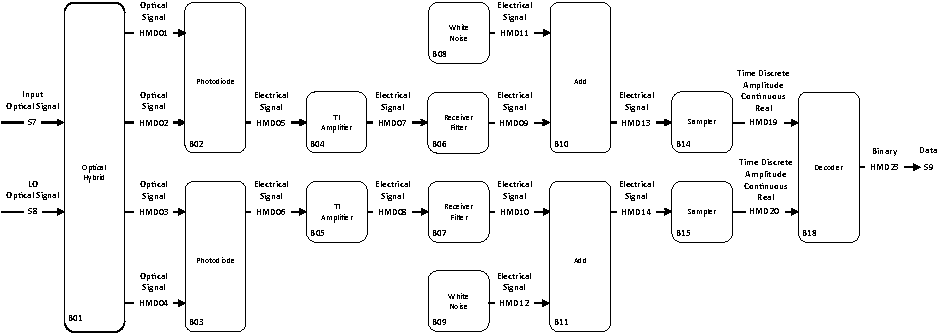
\includegraphics[width=\textwidth]{../lib/m_qam_receiver/figures/homodyneRx_blocks.pdf}
	\caption{Schematic representation of the block homodyne
	receiver.}\label{fig:homodyneRx_blocks}
\end{figure}

\subsection*{Input parameters}

This block input parameters that can be manipulated by the user in
order to change the configuration of the receiver. Each parameter is changed by
calling a
particular function. In the following table
(Table~\ref{tab:homodyneRx_params}) the input parameters and corresponding
functions are
summarized.
%
\begin{table}[h]
	\begin{center}
		\begin{tabular}{| m{3,2cm} | m{6,2cm} |  m{2,2cm} | m{4cm} | }
			\hline
			\textbf{Input parameters} & \textbf{Function} & \textbf{Type} &
			\textbf{Accepted values} \\ \hline
			IQ amplitudes & setIqAmplitudes & Vector of coordinate points in the I-Q
			plane & \textbf{Example} for a 4-QAM mapping: \{ \{ 1.0, 1.0 \}, \{ -1.0,
			1.0 \}, \{ -1.0, -1.0 \}, \{ 1.0, -1.0 \} \} \\ \hline
			Local oscillator power (in dBm) & setLocalOscillatorOpticalPower\_dBm &
			double(t\_real) & Any double greater than zero\\ \hline
			Local oscillator phase & setLocalOscillatorPhase & double(t\_real) & Any
			double greater than zero\\ \hline
			Responsivity of the photodiodes & setResponsivity & double(t\_real)
			&$\in$ [0,1] \\ \hline
			Amplification (of the TI amplifier) & setAmplification & double(t\_real)
			& Positive real number\\ \hline
			Noise amplitude (introduced by the TI amplifier) & setNoiseAmplitude &
			double(t\_real) & Real number greater than zero \\ \hline
			Samples to skip & setSamplesToSkip & int(t\_integer) &  \\ \hline
			Save internal signals & setSaveInternalSignals & bool & True or False\\
			\hline
			Sampling period & setSamplingPeriod & double & Given by $\frac{
			\textit{symbolPeriod}}{\textit{samplesPerSymbol}}$\\
			\hline
		\end{tabular}
		\caption{List of input parameters of the block MQAM receiver}
		\label{tab:homodyneRx_params}
	\end{center}
\end{table}
%
%\pagebreak

\subsection*{Methods}

%HomodyneReceiver(vector$<$Signal *$>$ \&inputSignal, vector$<$Signal *$>$
%\&outputSignal) (\textbf{constructor})
%\bigbreak
%void setIqAmplitudes(vector$<$t\_iqValues$>$ iqAmplitudesValues)
%\bigbreak
%vector$<$t\_iqValues$>$ const getIqAmplitudes(void)
%\bigbreak
%void setLocalOscillatorSamplingPeriod(double sPeriod)
%\bigbreak
%void setLocalOscillatorOpticalPower(double opticalPower)
%\bigbreak
%void setLocalOscillatorOpticalPower\_dBm(double opticalPower\_dBm)
%\bigbreak
%void setLocalOscillatorPhase(double lOscillatorPhase)
%\bigbreak
%void setLocalOscillatorOpticalWavelength(double lOscillatorWavelength)
%\bigbreak
%void setSamplingPeriod(double sPeriod)
%\bigbreak
%void  setResponsivity(t\_real Responsivity)
%\bigbreak
%void setAmplification(t\_real Amplification)
%\bigbreak
%void setNoiseAmplitude(t\_real NoiseAmplitude)
%\bigbreak
%void setImpulseResponseTimeLength(int impResponseTimeLength)
%\bigbreak
%void setFilterType(PulseShaperFilter fType)
%\bigbreak
%void setRollOffFactor(double rOffFactor)
%\bigbreak
%void setClockPeriod(double per)
%\bigbreak
%void setSamplesToSkip(int sToSkip)
%
%\pagebreak

\subsection*{Input Signals}

\subparagraph*{Number:} 2

\subparagraph*{Type:} Optical signal

\subsection*{Output Signals}

\subparagraph*{Number:} 1

\subparagraph*{Type:} Binary signal

\subsection*{Example}

\subparagraph*{Receiver sensitivity:}

The code was run several times for different noise powers of Thermal Noise and for each of them the BER was calculated and it is shown in table \ref{BER_TABLE1}. For noise power values above 1 mW, the signal is pratically lost since the BER is higher than 30\%.

In figure \ref{EyeDiagramThermal_a} it is possible to see that the eye diagram it\'s completely lost and in \ref{EyeDiagramThermal_b} it\'s still possible to see the optimal decision instant and that there is still a margin of error from each decision level.

\begin{figure}[H]
	\centering
        \begin{subfigure}{.45\textwidth}
        \centering
        	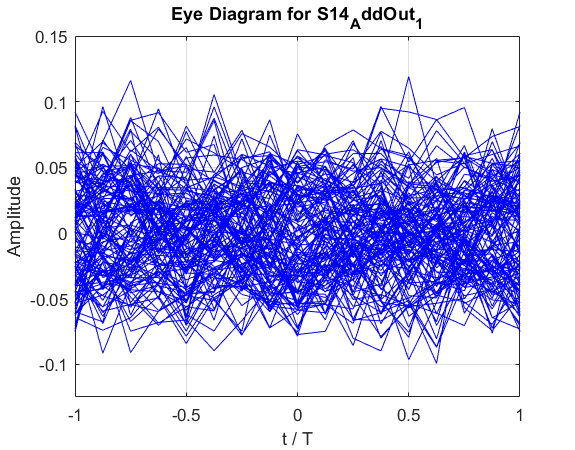
\includegraphics[scale=0.45]{./lib/m_qam_receiver/figures/Thermal5e-4.png}
        	\caption{Eye Diagram of Photodiode Sensor \newline with high thermal noise [1 mW]}\label{EyeDiagramThermal_a}
        \end{subfigure}%
        \begin{subfigure}{.45\textwidth}
        \centering
        	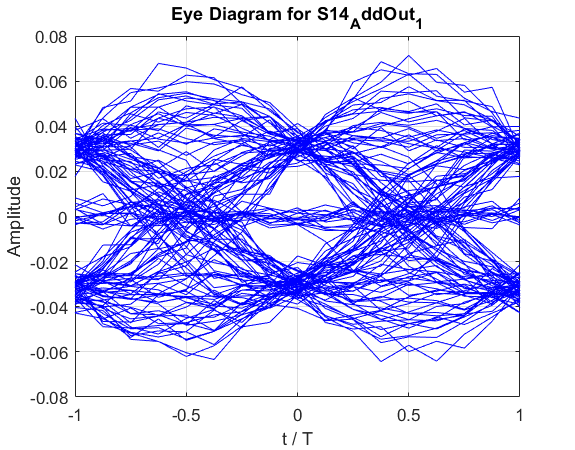
\includegraphics[scale=0.45]{./lib/m_qam_receiver/figures/Thermal1e-5.png}
        	\caption{Eye Diagram of Photodiode Sensor \newline with low thermal noise [10 uW]}\label{EyeDiagramThermal_b}
        \end{subfigure}
        \caption{Eye Diagrams from the Photodiode Sensor}\label{EyeDiagramThermal}
\end{figure}

\begin{table}[h]
\begin{center}
	\begin{tabular}{| c | c | }
		\hline
		\textbf{Thermal Noise Power} & \textbf{Bit error rate} \\ \hline
        1,00E-03 & 0.158898 \\ \hline
        5,00E-04 & 0.0677966 \\ \hline
        2,00E-04 & 0.0105932 \\ \hline
        1,00E-04 & 0.00317797 \\ \hline
        1,00E-05 & 0 \\ \hline
	\end{tabular}
	\caption{Impact on the Bit Error Rate from Thermal Noise} \label{BER_TABLE1}
\end{center}
\end{table}

\subparagraph*{Impact of the electrical amplifier:}

The code was run several times for different noise powers of white gaussian noise and for each of them the BER was calculated and it is shown in table \ref{BER_TABLE2}. For noise power values above 1e-16 W, the signal is pratically lost since the BER is higher than 30\%.

In figure \ref{EyeDiagramAmp_a} it is possible to see that the eye diagram it\'s completely lost and in \ref{EyeDiagramAmp_b} it\'s still possible to see the optimal decision instant and that there is almost no margin of error from each decision level.

This system has a gain of 1 by default and it\'s bandwidth is of 50 MHz has shown in figure \ref{ReceiverAmplifierFilter}.

\begin{figure}[H]
	\centering
        \begin{subfigure}{.45\textwidth}
        \centering
        	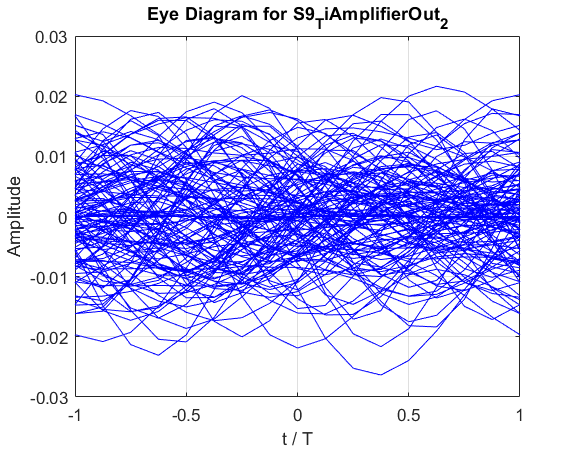
\includegraphics[width=.9\textwidth]{./lib/m_qam_receiver/figures/Amp5e-16.png}
        	\caption{Eye Diagram of Amplifier block \newline with high white gaussian noise power [5e-16 W]}\label{EyeDiagramAmp_a}
        \end{subfigure}%
        \begin{subfigure}{.45\textwidth}
        \centering
        	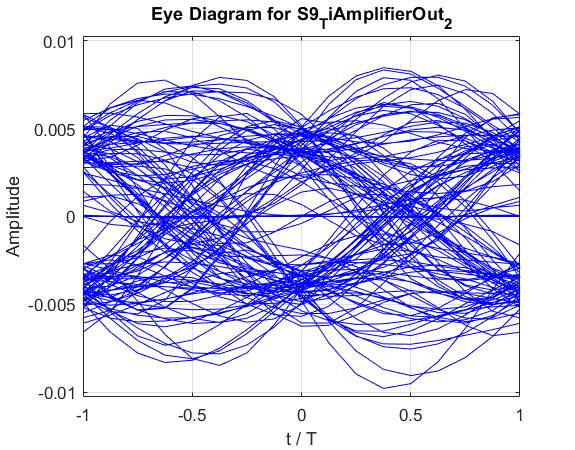
\includegraphics[width=.9\textwidth]{./lib/m_qam_receiver/figures/Amp1e-17.png}
        	\caption{Eye Diagram of Amplifier block \newline with low white gaussian noise power [1e-17 W]}\label{EyeDiagramAmp_b}
        \end{subfigure}
        \caption{Eye Diagrams from the Ti Amplifier}\label{EyeDiagramAmp}
\end{figure}

\begin{table}[h]
\begin{center}
	\begin{tabular}{| c | c | }
		\hline
		\textbf{Amplifier Noise Power} & \textbf{Bit error rate} \\ \hline
        1,00E-15 & 0.293432 \\ \hline
        5,00E-16 & 0.231992 \\ \hline
        2,00E-16 & 0.112288 \\ \hline
        1,00E-16 & 0.0370763 \\ \hline
        1,00E-17 & 0 \\ \hline
	\end{tabular}
	\caption{Impact on the Bit Error Rate from the Amplifier white gaussian noise} \label{BER_TABLE2}
\end{center}
\end{table}

\begin{figure}[h]
	\centering
    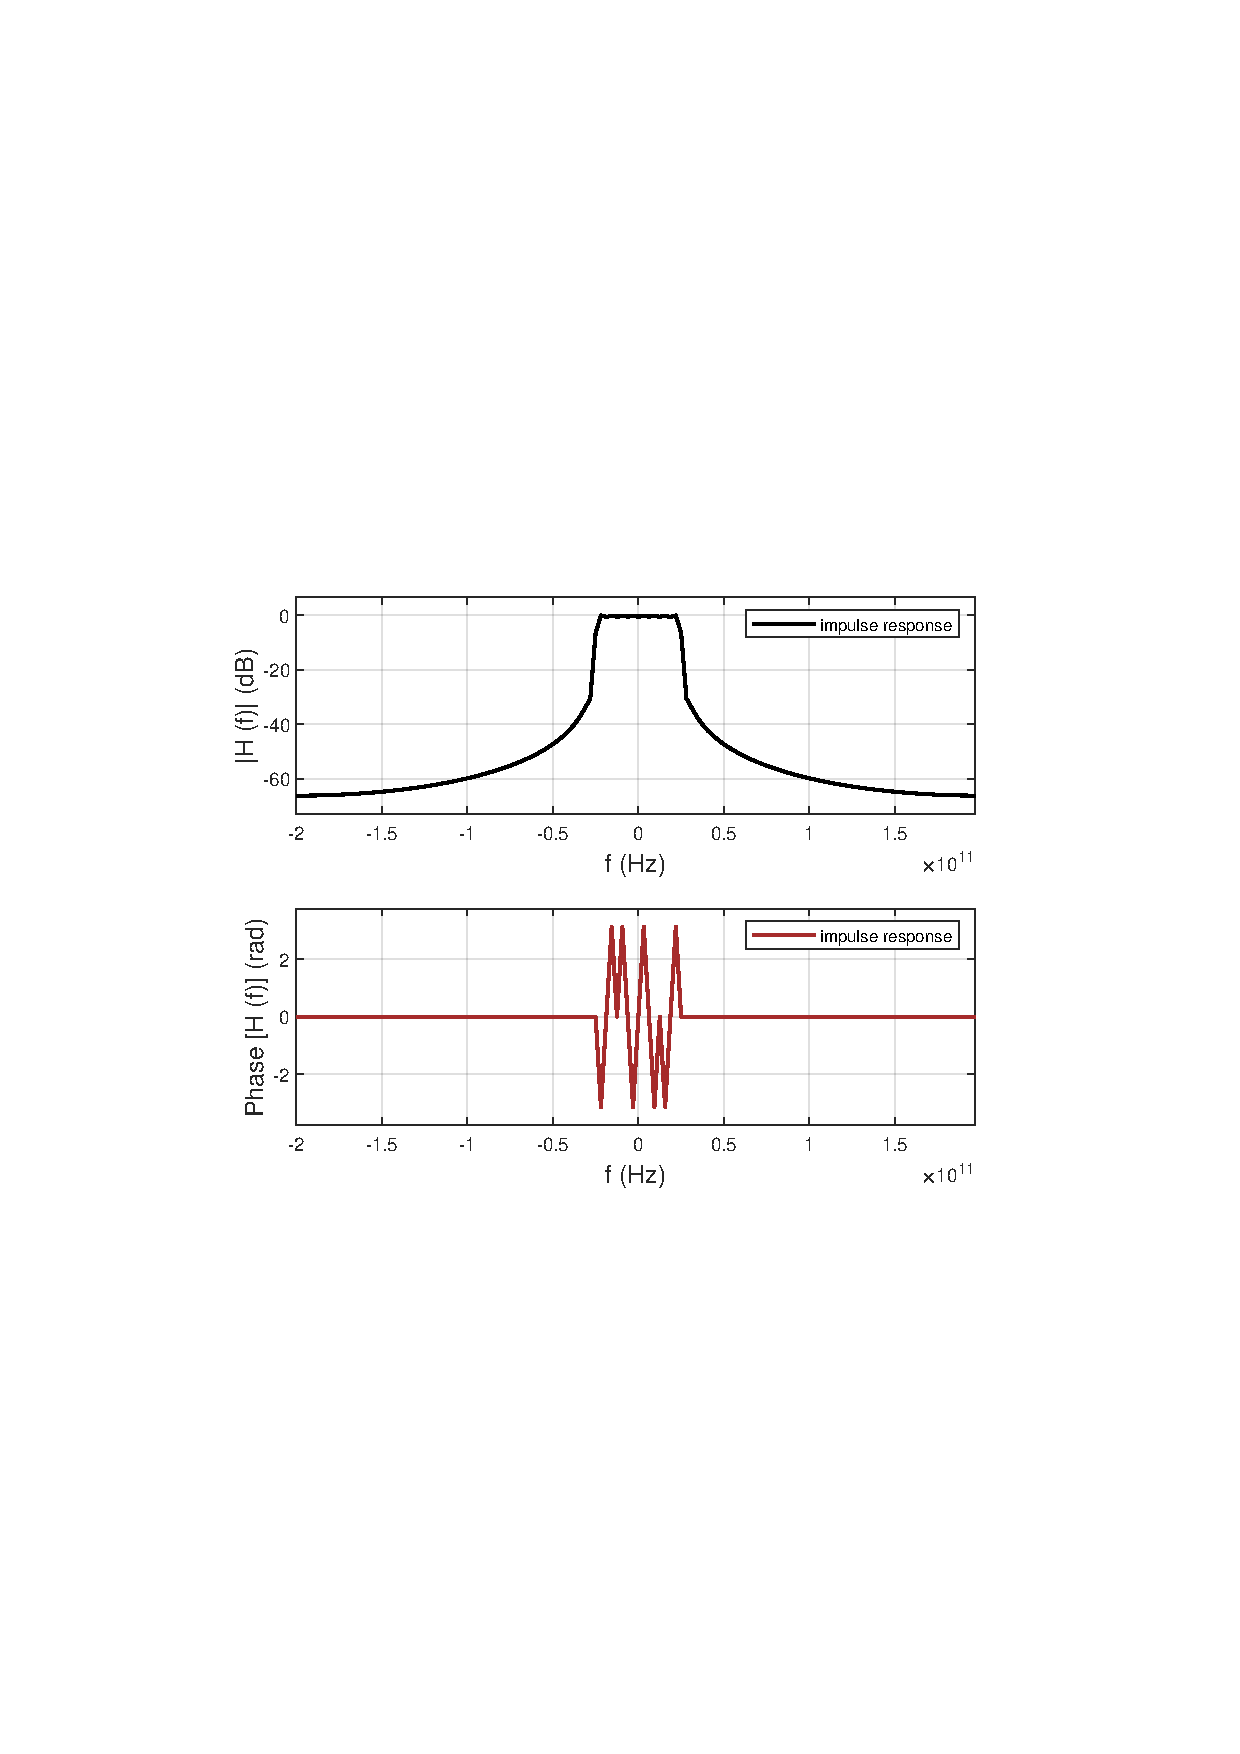
\includegraphics[clip, trim=0.5cm 9cm 0.5cm 9cm, width=\textwidth]{./lib/m_qam_receiver/figures/Filter.pdf}
    \caption{Ti Amplifier filter amplitude and phase}\label{ReceiverAmplifierFilter}
\end{figure}

\subsection*{Suggestions for future improvement}
